% ********************************************* %
%    Template 0.1, David Auzinger, 17.07.2015
% ********************************************* %

\documentclass[11pt, a4paper]{scrartcl} 	%Dokumententype und Schriftgröße
\usepackage[naustrian]{babel}  				%Sprache Österreichisch
\RequirePackage{ifthen}						%If then Package für Abfragen

\usepackage{lmodern}		 				%Latin Modern Fonts
\usepackage[T1]{fontenc}					%Schriften unterschiedlicher Kodierung
\usepackage[utf8]{inputenc}					%Eingabekodierung UTF8
\usepackage{amsmath}
\usepackage{listingsutf8}					%Listings Package

\usepackage{parskip} 			%Abstand zwiscthen Absätzen
\usepackage{fancyhdr}			%Kopf / Fußzeilen befüllen
\usepackage{graphicx}			%Lib für das Einbinden von Bildern
\usepackage{geometry}			%Einstellen von den Gemetrien des Dokuments
\usepackage{float}				%Bild an eine fixe Position legen
\usepackage{textcomp}			%Für UTF8 listign
\usepackage{listings}			%Code Lisiting in Latex
\usepackage{esdiff}				%Aufrechtes Symbol beim Differenzieren
\usepackage{amsmath}			%Mathematik Umgebung
\usepackage{longtable}			%Erweiterung für Mehrseitige Tabellen
\usepackage{titlesec}			%Zum setzen von Titelabständen
\usepackage{siunitx} 			%SI Units
\usepackage{trfsigns}			%Komplexe Zeichen (Laplace hantln und so sachen)
\usepackage{pdfpages}			%Einbinden von PDF Seiten
\usepackage{epstopdf}			%EPS grafiken
\usepackage{tabularx}			%Für mehrzeilige Tabelleneinträge
\usepackage{trfsigns}			%Laplace Trafo  
\usepackage{etoolbox}			%\ifdef

\usepackage{hyperref}			%Sprungmarken in PDF Datei einfügen

\usepackage{ecgdraw} % draw ecg-curves

\usepackage{subcaption}
\usepackage[breakable, theorems, skins]{tcolorbox}
\tcbset{enhanced}

\definecolor{exkboxcolor}{RGB}{255,220,220}
\DeclareRobustCommand{\exkbox}[2][exkboxcolor]{%
	\begin{tcolorbox}[   %% Adjust the following parameters at will.
		breakable,
		left=0pt,
		right=0pt,
		top=0pt,
		bottom=0pt,
		colback=#1,
		colframe=#1,
		width=\dimexpr0.95\textwidth\relax, 
		enlarge left by=5mm,
		boxsep=5pt,
		arc=0pt,outer arc=0pt,
		]
		#2
	\end{tcolorbox}
}

\definecolor{bspboxcolor}{RGB}{230,230,255}
\DeclareRobustCommand{\bspbox}[2][bspboxcolor]{%
	\begin{tcolorbox}[   %% Adjust the following parameters at will.
		breakable,
		left=0pt,
		right=0pt,
		top=0pt,
		bottom=0pt,
		colback=#1,
		colframe=#1,
		width=\dimexpr0.95\textwidth\relax, 
		enlarge left by=5mm,
		boxsep=5pt,
		arc=0pt,outer arc=0pt,
		]
		#2
	\end{tcolorbox}
}

%---------------------------------- 
% Dokumentparameter 
%----------------------------------

%\newcommand{\commercial}{}

% Author Information
\newcommand{\varAuthOneName}		{David Auzinger}
\newcommand{\varAuthOneInstitution}	{ASBÖ Linz}
\newcommand{\varAuthTwoName}		{\textbf{Inoffiziell, ohne Gewähr!}}

% Date
%\day=1 \month=1 \year=2015  

\title{EKG Erste Schritte \& Basiskurs}
\author{
\ifdef{\varAuthOneName}{\varAuthOneName\ifdef{\varAuthOneInstitution}{ - \varAuthOneInstitution}{}}{}
\ifdef{\varAuthTwoName}{\\\varAuthTwoName\ifdef{\varAuthTwoInstitution}{ - \varAuthTwoInstitution}{}}{}
\ifdef{\varAuthThreeName}{\\\varAuthThreeName\ifdef{\varAuthThreeInstitution}{ - \varAuthThreeInstitution}{}}{}
}


%----------------------------------
% Kopf / Fußnote 
%----------------------------------
\geometry{top=20mm, left=20mm, right=20mm, bottom=40mm}
%\reversemarginpar							%Margin Seiten Vertauschen
%\setlength{\headwidth}{170mm}
%\setlength{\headsep}{25mm}
\setlength{\headheight}{15mm}
%\setlength{\marginparwidth}{30mm}
%\setlength{\oddsidemargin}{30mm}
%\setlength{\textheight}{223mm}
%\setlength{\textwidth}{135mm}

\fancyhf{} %alle Kopf- und Fußzeilenfelder bereinigen
\renewcommand{\headrulewidth}{0.5pt}
\renewcommand{\footrulewidth}{0.5pt}
\lhead{EKG Erste Schritte \& Basiskurs}
\chead{}
\rhead{\subtitle} 
\lfoot{}
\cfoot{
\ifdef{\varAuthOneName}{\varAuthOneName}{}
\ifdef{\varAuthTwoName}{ | \varAuthTwoName}{}
\ifdef{\varAuthThreeName}{ | \varAuthThreeName}{}
}
\rfoot{\thepage}


 
%-------------------------------------------
% Listings konfiguration
%-------------------------------------------
%Compuler XE LATEX = true
\lstset{
basicstyle=\ttfamily\footnotesize,, 
numbers=left, 
language=Matlab,
showstringspaces=false,
breaklines=true,
breakautoindent=true, 
tabsize=2, 
frame=single,
literate=%
	{Ö}{{\"O}}1
	{Ä}{{\"A}}1
	{Ü}{{\"U}}1
	{ß}{{\ss}}2
	{ü}{{\"u}}1
	{ä}{{\"a}}1
	{ö}{{\"o}}1
}



%-------------------------------------------
% TitelEinstellungen 
%-------------------------------------------
%\renewcommand*{\thesubsection}{\alph{subsection})} 
%\renewcommand*{\thesubsubsection}{\alph{subsection}\alph{subsubsection})} 
%\makeatletter 

%\titlespacing*{\section}{0pt}{0pt}{15pt}
%\titlespacing*{\subsection}{0pt}{0pt}{-15pt}

\newcommand{\unit}{\SI}

\begin{document}

%----------------------------------
% Automatisierte Ausgaben
%----------------------------------



\pagestyle{fancy}


%Titelblatt
\maketitle

\vspace{3cm}



\newpage

%Inhaltsverzeichnis
\tableofcontents
\newpage

% Include predefined EKG-Curves
%%
%% This is file `archivio.tex',
%% generated with the docstrip utility.
%%
%% The original source files were:
%%
%% ecgdraw.dtx  (with options: `archivio')
%% ________________________________________
%% A package to draw ECG.
%% Copyright (C) 2016 Marco Scavino and Ezio Aimé
%% All rights reserved
%% License information appended
%\ProvidesFile{archivio}[2015/08/31 v.1.0 Draw ECG]
\nuovoECG{d1}{(1cm,0)node[left]{I}}
\nuovoECG{d2}{(1cm,0)node[left]{II}}
\nuovoECG{d3}{(1cm,0)node[left]{III}}
\nuovoECG{vr}{(1cm,0)node[left]{aVR}}
\nuovoECG{vl}{(1cm,0)node[left]{aVL}}
\nuovoECG{vf}{(1cm,0)node[left]{aVF}}
\nuovoECG{v1}{(1cm,0)node[left]{V1}}
\nuovoECG{v2}{(1cm,0)node[left]{V2}}
\nuovoECG{v3}{(1cm,0)node[left]{V3}}
\nuovoECG{v4}{(1cm,0)node[left]{V4}}
\nuovoECG{v5}{(1cm,0)node[left]{V5}}
\nuovoECG{v6}{(1cm,0)node[left]{V6}}

\nuovoECG{tara}{(0,0)--(.1,0)--(.1,1)--(.5,1)--(.5,0)--(1,0)}

\nuovoECG{pp0160}{(0,0)--(.04,.06)--(.085,.1)--(.12,.06)--(.15,.0)}
\nuovoECG{pp0260}{(0,0)--(.02,.1)--(.085,.2)--(.13,.1)--(.15,.0)}
\nuovoECG{pp0360}{(0,0)--(.04,.2)--(.085,.3)--(.12,.2)--(.15,.0)}
\nuovoECG{pp0180}{(0,0)--(.04,.06)--(.09,.1)--(.14,.06)--(.2,.0)}
\nuovoECG{pp0280}{(0,0)--(.02,.1)--(.09,.2)--(.15,.1)--(.2,.0)}
\nuovoECG{pp0380}{(0,0)--(.04,.2)--(.09,.3)--(.14,.2)--(.2,.0)}
\nuovoECG{pp0199}{(0,0)--(.1,.08)--(.15,.1)--(.2,.08)--(.25,.0)}
\nuovoECG{pp0299}{(0,0)--(.1,.16)--(.15,.2)--(.2,.16)--(.25,.0)}
\nuovoECG{pp0399}{(0,0)--(.1,.2)--(.15,.3)--(.2,.2)--(.25,.0)}

\nuovoECG{pn0160}{(0,0)--(.04,-.06)--(.085,-.1)--(.12,-.06)--(.15,.0)}
\nuovoECG{pn0260}{(0,0)--(.02,-.1)--(.085,-.2)--(.13,-.1)--(.15,.0)}
\nuovoECG{pn0360}{(0,0)--(.04,-.2)--(.085,-.3)--(.12,-.2)--(.15,.0)}
\nuovoECG{pn0180}{(0,0)--(.04,-.06)--(.09,-.1)--(.14,-.06)--(.2,.0)}
\nuovoECG{pn0280}{(0,0)--(.02,-.1)--(.09,-.2)--(.15,-.1)--(.2,.0)}
\nuovoECG{pn0380}{(0,0)--(.04,-.2)--(.09,-.3)--(.14,-.2)--(.2,.0)}
\nuovoECG{pn0199}{(0,0)--(.1,-.08)--(.15,-.1)--(.2,-.08)--(.25,.0)}
\nuovoECG{pn0299}{(0,0)--(.1,-.16)--(.15,-.2)--(.2,-.16)--(.25,.0)}
\nuovoECG{pn0399}{(0,0)--(.1,-.2)--(.15,-.3)--(.2,-.2)--(.25,.0)}

\nuovoECG{pd1199}{(0,0)--(0.01,0.005)--(0.09,0.095)--(0.11,0.095)
 --(0.19,-0.095)--(0.21,-0.095)--(0.29,-0.005)--(0.3,0)}
\nuovoECG{pb2199}{(0,0)--(0.01,0.005)--(0.09,0.195)--(0.11,0.195)--(0.14,0.1)
 --(0.16,0.1)--(0.19,0.15)--(0.21,0.15)--(0.29,0.005)-- (0.3,0)}
\nuovoECG{pb1299}{(0,0)--(0.01,0.005)--(0.09,0.15)--(0.11,0.15)--(0.14,0.1)
 --(0.16,0.1)--(0.19,0.195)--(0.21,0.195)--(0.29,0.005)-- (0.3,0)}

\nuovoECG{q21}{(0,0)--(.025,-.1)--(.05,0)}
\nuovoECG{q22}{(0,0)--(.025,-.2)--(.05,0)}
\nuovoECG{q23}{(0,0)--(.025,-.3)--(.05,0)}

\nuovoECG{q41}{(0,0)--(.05,-.1)--(.1,0)}
\nuovoECG{q42}{(0,0)--(.05,-.2)--(.1,0)}
\nuovoECG{q43}{(0,0)--(.05,-.3)--(.1,0)}
\nuovoECG{q44}{(0,0)--(.05,-.4)--(.1,0)}
\nuovoECG{q45}{(0,0)--(.05,-.5)--(.1,0)}

\nuovoECG{r31}{(0,0)--(.035,.1)--(.075,0)}
\nuovoECG{r32}{(0,0)--(.035,.2)--(.075,0)}
\nuovoECG{r33}{(0,0)--(.035,.3)--(.075,0)}
\nuovoECG{r34}{(0,0)--(.035,.4)--(.075,0)}
\nuovoECG{r35}{(0,0)--(.035,.5)--(.075,0)}

\nuovoECG{r42}{(0,0)--(.05,.2)--(.1,0)}
\nuovoECG{r44}{(0,0)--(.05,.4)--(.1,0)}
\nuovoECG{r46}{(0,0)--(.05,.6)--(.1,0)}
\nuovoECG{r48}{(0,0)--(.05,.8)--(.1,0)}
\nuovoECG{r100}{(0,0)--(.05,1)--(.1,0)}

\nuovoECG{r412}{(0,0)--(.05,1.2)--(.1,0)}
\nuovoECG{r416}{(0,0)--(.05,1.6)--(.1,0)}
\nuovoECG{r420}{(0,0)--(.05,2)--(.1,0)}
\nuovoECG{r424}{(0,0)--(.05,2.4)--(.1,0)}
\nuovoECG{r428}{(0,0)--(.05,2.8)--(.1,0)}
\nuovoECG{r432}{(0,0)--(.05,3.2)--(.1,0)}

\nuovoECG{r510}{(0,0)--(.0625,1)--(.125,0)}
\nuovoECG{r515}{(0,0)--(.0625,1.5)--(.125,0)}
\nuovoECG{r520}{(0,0)--(.0625,2)--(.125,0)}
\nuovoECG{r525}{(0,0)--(.0625,2.5)--(.125,0)}
\nuovoECG{r530}{(0,0)--(.0625,3)--(.125,0)}
\nuovoECG{r535}{(0,0)--(.0625,3.5)--(.125,0)}
\nuovoECG{r540}{(0,0)--(.0625,4)--(.125,0)}
\nuovoECG{r545}{(0,0)--(.0625,4.5)--(.125,0)}

\nuovoECG{s31}{(0,0)--(.035,-.1)--(.075,0)}
\nuovoECG{s32}{(0,0)--(.035,-.2)--(.075,0)}
\nuovoECG{s33}{(0,0)--(.035,-.3)--(.075,0)}
\nuovoECG{s34}{(0,0)--(.035,-.4)--(.075,0)}
\nuovoECG{s35}{(0,0)--(.035,-.5)--(.075,0)}

\nuovoECG{s42}{(0,0)--(.05,-.2)--(.1,0)}
\nuovoECG{s44}{(0,0)--(.05,-.4)--(.1,0)}
\nuovoECG{s46}{(0,0)--(.05,-.6)--(.1,0)}
\nuovoECG{s48}{(0,0)--(.05,-.8)--(.1,0)}
\nuovoECG{s410}{(0,0)--(.05,-1)--(.1,0)}

\nuovoECG{s412}{(0,0)--(.05,-1.2)--(.1,0)}
\nuovoECG{s416}{(0,0)--(.05,-1.6)--(.1,0)}
\nuovoECG{s420}{(0,0)--(.05,-2)--(.1,0)}
\nuovoECG{s424}{(0,0)--(.05,-2.4)--(.1,0)}
\nuovoECG{s428}{(0,0)--(.05,-2.8)--(.1,0)}
\nuovoECG{s432}{(0,0)--(.05,-3.2)--(.1,0)}

\nuovoECG{s510}{(0,0)--(.0625,-1)--(.125,0)}
\nuovoECG{s515}{(0,0)--(.0625,-1.5)--(.125,0)}
\nuovoECG{s520}{(0,0)--(.0625,-2)--(.125,0)}
\nuovoECG{s525}{(0,0)--(.0625,-2.5)--(.125,0)}
\nuovoECG{s530}{(0,0)--(.0625,-3)--(.125,0)}
\nuovoECG{s535}{(0,0)--(.0625,-3.5)--(.125,0)}
\nuovoECG{s540}{(0,0)--(.0625,-4)--(.125,0)}
\nuovoECG{s545}{(0,0)--(.0625,-4.5)--(.125,0)}

\nuovoECG{tp2}{(0,0)--(.2,.05)--(.3,.15)--(.45,.2)--(.55,.2)--(.7,.15)--(.8,.05)--(1,0)}
\nuovoECG{tp3}{(0,0)--(.2,.085)--(.3,.18)--(.45,.3)--(.55,.3)--(.7,.18)--(.8,.085)--(1,0)}
\nuovoECG{tp4}{(0,0)--(.1,.03)-- (.2,.12)--(.3,.25)--(.45,.4)--(.55,.4)--(.7,.25)--(.8,.12)--(.9,.06)--(1,0)}
\nuovoECG{tp5}{(0,0)--(.1,.03)--(.2,.13)--(.3,.29)--(.4,.47)--(.45,.5)--(.55,.5)--(.6,.47)--(.7,.29)--(.8,.13)--(.9,.03)--(1,0)}
\nuovoECG{tp6}{(0,0)--(.1,.04)--(.2,.19)--(.3,.36)--(.4,.53)--(.45,.6)--(.55,.6)--(.6,.53)--(.7,.36)--(.8,.19)--(.9,.04)--(1,0)}
\nuovoECG{tp7}{(0,0)--(.1,.04)--(.2,.2)--(.3,.39)--(.4,.58)--(.45,.7)--(.55,.7)--(.6,.58)--(.7,.39)--(.8,.2)--(.9,.04)--(1,0)}
\nuovoECG{tp8}{(0,0)--(.1,.04)--(.2,.21)--(.3,.45)--(.4,.67)--(.45,.8)--(.55,.8)--(.6,.67)--(.7,.45)--(.8,.21)--(.9,.04)--(1,0)}
\nuovoECG{tp9}{(0,0)--(.1,.05)--(.2,.4)--(.3,.62)--(.4,.85)--(.45,.9)--(.55,.85)--(.7,.62)--(.8,.4)--(.9,.05)--(1,0)}
\nuovoECG{tp10}{(0,0)--(.1,.05)--(.2,.42)--(.3,.66)--(.4,.9)--(.45,1)--(.55,1)--(.6,.9)--(.7,.66)--(.8,.42)--(.9,.05)--(1,0)}
\nuovoECG{tp11}{(0,0)--(.1,.05)--(.2,.48)--(.3,.73)--(.4,.97)--(.45,1.1)--(.55,1.1)--(.6,.97)--(.7,.73)--(.8,.48)--(.9,.05)--(1,0)}

\nuovoECG{tn2}{(0,0)--(.2,-.05)--(.3,-.15)--(.45,-.2)--(.55,-.2)--(.7,-.15)--(.8,-.05)--(1,0)}
\nuovoECG{tn3}{(0,0)--(.2,-.085)--(.3,-.18)--(.45,-.3)--(.55,-.3)--(.7,-.18)--(.8,-.085)--(1,0)}
\nuovoECG{tn4}{(0,0)--(.1,-.03)-- (.2,-.12)--(.3,-.25)--(.45,-.4)--(.55,-.4)--(.7,-.25)--(.8,-.12)--(.9,-.06)--(1,0)}
\nuovoECG{tn5}{(0,0)--(.1,-.03)--(.2,-.13)--(.3,-.29)--(.4,-.47)--(.45,-.5)--(.55,-.5)--(.6,-.47)--(.7,-.29)--(.8,-.13)--(.9,-.03)--(1,0)}
\nuovoECG{tn6}{(0,0)--(.1,-.04)--(.2,-.19)--(.3,-.36)--(.4,-.53)--(.45,-.6)--(.55,-.6)--(.6,-.53)--(.7,-.36)--(.8,-.19)--(.9,-.04)--(1,0)}
\nuovoECG{tn7}{(0,0)--(.1,-.04)--(.2,-.2)--(.3,-.39)--(.4,-.58)--(.45,-.7)--(.55,-.7)--(.6,-.58)--(.7,-.39)--(.8,-.2)--(.9,-.04)--(1,0)}
\nuovoECG{tn8}{(0,0)--(.1,-.04)--(.2,-.21)--(.3,-.45)--(.4,-.67)--(.45,-.8)--(.55,-.8)--(.6,-.67)--(.7,-.45)--(.8,-.21)--(.9,-.04)--(1,0)}
\nuovoECG{tn9}{(0,0)--(.1,-.05)--(.2,-.4)--(.3,-.62)--(.4,-.85)--(.45,-.9)--(.55,-.85)--(.7,-.62)--(.8,-.4)--(.9,-.05)--(1,0)}
\nuovoECG{tn10}{(0,0)--(.1,-.05)--(.2,-.42)--(.3,-.66)--(.4,-.9)--(.45,-1)--(.55,-1)--(.6,-.9)--(.7,-.66)--(.8,-.42)--(.9,-.05)--(1,0)}
\nuovoECG{tn11}{(0,0)--(.1,-.05)--(.2,-.48)--(.3,-.73)--(.4,-.97)--(.45,-1.1)--(.55,-1.1)--(.6,-.97)--(.7,-.73)--(.8,-.48)--(.9,-.05)--(1,0)}

\nuovoECG{nnd1}{(0,0)--(.1,.08)--(.18,0)--(.3,0)--(.4,-.1)--(.42,.8)--(.48,.1)--(.55,0)--(.8,0)--(.9,.1)--(1,.2)--(1.1,.3)--(1.2,.2)--(1.3,0)--(1.8,0)}
\nuovoECG{nnd2}{(0,0)--(.05,.05)--(.08,.1)--(.15,.05)--(.2,0)--(.3,0)--(.35,-.1)--(.4,.9)--(.5,-.02)--(.6,0)--(.9,0)--(1,.1)--(1.1,.2)--(1.15,.3)--(1.25,.2)--(1.3,.05)--(1.8,0)}
\nuovoECG{nnd3}{(0,0)--(0.08,0.05)--(0.15,0.02)--(0.3,0)--(0.4,0.08)--(0.43,0.21)--(0.48,-0.1)--(0.52,0)--(1.05,0)--(1.1,0.07)--(1.2,0)--(1.8,0)}
\nuovoECG{nnvr}{(0,0)--(0.08,-0.05)--(0.12,-0.14)--(0.2,0)--(0.3,0)--(0.4,0.01)--(0.43,0.08)--(0.48,-0.9)--(0.52,-0.1)--(0.8,0)--(0.9,-0.1)--(1,-0.2)--(1.1,-0.3)--(1.15,-0.3)--(1.25,-0.1)--(1.3,0)--(1.5,0)}
\nuovoECG{nnvl}{(0,0)--(0.08,-0.05)--(0.16,0.1)--(0.21,0)--(0.4,0)--(0.41,-0.01)--(0.45,0.38)--(0.55,0.05)--(0.6,0)--(0.8,0)--(0.9,0.05)--(1,0.1)--(1.1,0.18)--(1.2,0.05)--(1.3,0)--(1.5,0)}
\nuovoECG{nnvf}{(0,0)--(0.1,0.05)--(0.17,-0.05)--(0.2,0)--(0.4,0)--(0.46,0.6)--(0.5,-0.1)--(0.55,0)--(.7,.02)--(.8,.03)--(0.9,.04)--(1.0,0.5)--(1.1,0.1)--(1.15,0.15)--(1.2,0.1)--(1.3,0)--(1.5,0)}

\nuovoECG{nnv1}{(0,0)--(0.08,0)--(0.1,0.05)--(0.17,0.1)--(0.2,-0.05)--(0.24,0)--(0.4,0)--(0.42,0.2)--(0.5,-1.1)--(0.6,0)--(0.7,0)--(0.8,0.08)--(0.9,0.1)--(1,0)--(1.1,-0.08)--(1.18,-0.1)--(1.2,-0.04)--(1.3,0)--(1.5,0)}
\nuovoECG{nnv2}{(0,0)--(.05,.05)--(.15,.2)--(.2,0)--(.4,0)--(.45,.3)--(.5,-.55)--(.6,0)--(.7,.08)--(.8,.12)--(.9,.2)--(1,.35)--(1.1,.5)--(1.2,.4)--(1.3,.05)--(1.5,0)}
\nuovoECG{nnv3}{(0,0)--(0.1,0)--(0.15,0.1)--(0.2,0)--(0.4,0)--(0.5,1)--(0.55,-0.1)--(0.6,0)--(0.7,0)--(0.8,0.05)--(0.9,0.1)--(1,0.3)--(1.1,0.6)--(1.15,0.7)--(1.2,0.4)--(1.3,0.1)--(1.4,0)--(1.6,0)}
\nuovoECG{nnv4}{(0,0)--(0.1,0)--(0.14,0.1)--(0.2,0)--(0.4,0)--(0.41,-0.07)--(0.5,1.35)--(0.55,-0.03)--(0.6,0)--(0.8,0)--(0.9,0.1)--(1,0.2)--(1.1,0.4)--(1.15,0.55)--(1.2,0.4)--(1.3,0.1)--(1.5,0)--(1.6,0)}
\nuovoECG{nnv5}{(0,0)--(0.1,0)--(0.15,0.1)--(0.2,0)--(0.4,0)--(0.45,-0.1)--(0.5,1.2)--(0.55,-0.05)--(0.6,0)--(0.8,0)--(0.9,0.05)--(1,0.1)--(1.1,0.3)--(1.2,0.4)--(1.3,0.02)--(1.4,0)--(1.6,0)}
\nuovoECG{nnv6}{(0,0)--(0.1,0)--(0.16,0.09)--(0.2,0)--(0.4,0)--(0.44,-0.09)--(0.5,0.9)--(0.55,0.01)--(0.6,0)--(0.9,0)--(1,0.1)--(1.1,0.2)--(1.18,0.34)--(1.2,0.25)--(1.3,0.1)--(1.4,0)--(1.6,0)}

\nuovoECG{nbd1}{(0,0)--(0.1,0.05)--(0.18,0)--(0.2,0.1)--(0.25,0)--(0.4,0)--(0.45,-0.1)--(0.5,0.9)--(0.6,-0.15)--(0.65,0)--(0.9,0)--(1,0.05)--(1.1,0.1)--(1.2,0.2)--(1.3,0.35)--(1.4,0.4)--(1.5,0.1)--(1.6,0)--(1.8,0)}
\nuovoECG{nbd2}{(0,0)--(0.1,0.08)--(0.2,0.12)--(0.3,0)--(0.5,0)--(0.6,0.02)--(0.7,0.75)--(0.8,-0.2)--(0.9,0)--(1.1,0)--(1.2,0.05)--(1.3,0.08)--(1.4,0.3)--(1.45,0.35)--(1.5,0.3)--(1.6,0.05)--(1.7,0)--(1.8,0)}
\nuovoECG{nbd3}{(0,0)--(0.05,0)--(0.1,0.05)--(0.15,0.1)--(0.2,0.05)--(0.3,0)--(0.4,0)--(0.5,0)--(0.6,0.1)--(0.7,-0.7)--(0.8,0)--(1.3,0)--(1.4,-0.08)--(1.5,0)--(1.6,0)--(1.8,0)}
\nuovoECG{nbvr}{(0,0)--(0.1,-0.05)--(0.2,-0.1)--(0.3,0)--(0.5,0)--(0.6,0.02)--(0.65,-0.8)--(0.7,0.2)--(0.8,0)--(1,0)--(1.1,-0.05)--(1.2,-0.1)--(1.3,-0.2)--(1.4,-0.3)--(1.5,-0.2)--(1.6,-0.1)--(1.7,0)--(1.8,0)}
\nuovoECG{nbvl}{(0,0)--(0.09,-0.05)--(0.16,-0.05)--(0.26,0.05)--(0.4,0)--(0.5,0)--(0.57,-0.1)--(0.65,0.8)--(0.7,-0.02)--(0.75,0)--(1.1,0)--(1.2,0.03)--(1.3,0.1)--(1.4,0.2)--(1.5,0.1)--(1.6,0.02)--(1.7,0)--(1.8,0)}
\nuovoECG{nbvf}{(0,0)--(0.09,0.1)--(0.16,0.12)--(0.2,0.02)--(0.3,0)--(0.5,0)--(0.6,0.1)--(0.65,0.3)--(0.7,-0.1)--(0.75,0)--(0.8,0.01)--(0.9,0.02)--(1,0.03)--(1.1,0.04)--(1.2,0.06)--(1.3,0.12)--(1.4,0.16)--(1.45,0.2)--(1.5,0.15)--(1.6,0.06)--(1.7,0.01)--(1.8,0)}

\nuovoECG{nbv1}{(0,0)--(0.1,0)--(0.2,-0.1)--(0.3,-0.04)--(0.4,0)--(0.5,0)--(0.58,0.12)--(0.66,-0.7)--(0.72,0.02)--(0.8,0)--(1.2,0)--(1.3,-0.04)--(1.4,-0.12)--(1.5,-0.15)--(1.6,0)--(1.8,0)}
\nuovoECG{nbv2}{(0,0)--(0.1,0)--(0.15,0.04)--(0.2,-0.04)--(0.3,0)--(0.5,0)--(0.58,0.75)--(0.65,-0.45)--(0.7,-0.2)--(0.75,0)--(1,0.01)--(1.1,0.1)--(1.2,0.2)--(1.3,0.3)--(1.4,0.45)--(1.5,0.3)--(1.6,0.08)--(1.7,0)--(1.8,0)}
\nuovoECG{nbv3}{(0,0)--(0.1,0.02)--(0.2,0.11)--(0.3,0)--(0.5,0)--(0.58,1.4)--(0.67,-0.6)--(0.7,-0.3)--(0.8,0.1)--(0.9,0.15)--(1.0,0.2)--(1.1,0.25)--(1.2,0.35)--(1.3,0.6)--(1.4,0.9)--(1.5,0.5)--(1.6,0.1)--(1.7,0)--(1.8,0)}
\nuovoECG{nbv4}{(0,0)--(0.1,0.03)--(0.16,0.1)--(0.2,0)--(0.3,0.05)--(0.4,0)--(0.5,0)--(0.58,2.2)--(0.68,-0.4)--(0.74,0)--(0.8,0.03)--(0.9,0.05)--(1,0.1)--(1.1,0.15)--(1.2,0.22)--(1.3,0.4)--(1.4,0.8)--(1.45,1)--(1.5,0.5)--(1.6,0.1)--(1.7,0.02)--(1.8,0)--(1.9,0)}
\nuovoECG{nbv5}{(0,0)--(0.1,0)--(0.2,0.03)--(0.3,0.08)--(0.4,0.02)--(0.5,0)--(0.6,0)--(0.63,-0.1)--(0.7,2.3)--(0.8,-0.3)--(0.85,0)--(0.9,0)--(1.0,0.02)--(1.1,0.08)--(1.2,0.1)--(1.3,0.2)--(1.4,0.4)--(1.5,0.8)--(1.6,0.5)--(1.7,0.1)--(1.8,0.05)--(1.9,0)--(2,0)}
\nuovoECG{nbv6}{(0,0)--(0.1,0.05)--(0.2,0.1)--(0.3,0.04)--(0.4,0)--(0.5,0)--(0.55,-0.12)--(0.6,1.9)--(0.7,-0.09)--(0.75,0)--(0.9,0)--(1,0.05)--(1.1,0.1)--(1.2,0.15)--(1.3,0.4)--(1.4,0.7)--(1.5,0.25)--(1.6,0.07)--(1.7,0)--(1.8,0)}

\nuovoECG{evd1}{(0,0)--(.1,0)--(.2,.15)--(.3,.1)--(.4,.44)--(.5,0)--(.7,0)--(.8,-.1)--(.9,0)--(1.0,.1)--(1.1,.15)--(1.2,-.05)--(1.3,-.02)--(1.4,0)--(1.5,0)}
\nuovoECG{evd2}{(0,0)--(.1,.05)--(.2,.5)--(.3,.9)--(.4,1.4)--(.5,.5)--(.6,-.15)--(.7,-.25)--(.8,-.35)--(.9,-.5)--(1.0,-.62)--(1.1,-.43)--(1.2,-.1)--(1.3,.04)--(1.4,0)--(1.5,0)}
\nuovoECG{evd3}{(0,0)--(.1,.05)--(.2,.1)--(.3,.7)--(.4,1.1)--(.45,1.35)--(.5,0)--(.6,-.2)--(.7,-.2)--(.8,-.3)--(.9,-.5)--(1,-.6)--(1.1,-.5)--(1.2,-.2)--(1.3,.1)--(1.4,.05)--(1.5,0)--(1.6,0)}
\nuovoECG{evvr}{(0,0)--(.1,0)--(.2,.05)--(.3,-.05)--(.4,-.05)--(.5,-.2)--(.6,-.5)--(.68,-.9)--(.7,-.7)--(.8,0)--(.9,.09)--(1,.12)--(1.1,.18)--(1.2,.2)--(1.3,.2)--(1.4,.16)--(1.5,.1)--(1.6,0)--(1.7,0)}
\nuovoECG{evvl}{(0,0)--(.1,0)--(.2,0)--(.3,.09)--(.4,-.3)--(.5,-.65)--(.6,0)--(.7,.05)--(.8,.1)--(.9,.2)--(1,.3)--(1.1,.4)--(1.15,.4)--(1.2,.3)--(1.3,0)--(1.4,-.1)--(1.5,0)--(1.6,0)}
\nuovoECG{evvf}{(0,0)--(0.1,.05)--(.2,.07)--(.3,.4)--(.4,.8)--(.5,1.32)--(.6,-.05)--(.7,-.18)--(.8,-.21)--(.9,-.3)--(1,-.5)--(1.1,-.67)--(1.2,-.05)--(1.3,-.01)--(1.4,.05)--(1.5,0)--(1.6,0)}

\nuovoECG{evv1}{(0,0)--(.2,0)--(.3,.02)--(.4,.4)--(.45,1)--(.5,.3)--(.55,-.2)--(.6,-.15)--(.7,-.25)--(.8,-.25)--(.9,-.3)--(1,-.4)--(1.1,-.5)--(1.2,-.3)--(1.3,0)--(1.6,0)}
\nuovoECG{evv2}{(0,0)--(.2,0)--(.3,.3)--(.4,1.6)--(.47,2.5)--(.5,1.7)--(.54,-.3)--(.6,-.25)--(.7,-.3)--(.8,-.35)--(.9,-.4)--(1,-.52)--(1.1,-.6)--(1.2,-.4)--(1.3,-.15)--(1.4,-.1)--(1.5,-.02)--(1.6,0)}
\nuovoECG{evv3}{(0,0)--(.2,0)--(.3,.7)--(.4,1.7)--(.46,2.8)--(.5,2.3)--(.6,0)--(.7,-.35)--(.8,-.4)--(.9,-.6)--(1,-.8)--(1.1,-1.05)--(1.2,-.8)--(1.3,-.3)--(1.4,-.05)--(1.5,0)--(1.6,0)}
\nuovoECG{evv4}{(0,0)--(.2,0)--(.3,.6)--(.4,1.7)--(.5,2.25)--(.6,-.2)--(.7,-.3)--(.8,-.45)--(.9,-.6)--(1,-.87)--(1.1,-1)--(1.2,-.6)--(1.3,-.2)--(1.4,-.1)--(1.5,-.04)--(1.55,0)--(1.6,0)}
\nuovoECG{evv5}{(0,0)--(.2,0)--(.3,.5)--(.4,1.5)--(.45,1.75)--(.5,1.1)--(.6,-.2)--(.7,-.28)--(.8,-.4)--(.9,-.5)--(1,-.7)--(1.07,-.8)--(1.1,-.7)--(1.2,-.4)--(1.3,-.2)--(1.4,-.1)--(1.5,0)--(1.6,0)}
\nuovoECG{evv6}{(0,0)--(.2,0)--(.3,.45)--(.4,1.3)--(.45,1.4)--(.5,.7)--(.6,-.1)--(.7,-.2)--(.8,-.25)--(.9,-.4)--(1,-.5)--(1.1,-.4)--(1.2,-.2)--(1.3,-.05)--(1.4,0)--(1.6,0)}

\nuovoECG{wbd1}{(0,0)--(.08,.07)--(.1,.04)--(.18,0)--(.2,-.02)--(.25,-.02)--(.26,0)--(.28,.22)--(.3,.15)--(.32,-.1)--(.4,0)--(.42,.02)--(.6,.05)--(.7,.12)--(.8,.19)--(.85,.05)--(.9,.02)--(1,.01)--(1.2,0)--(1.5,0)}
\nuovoECG{wbd2}{(0,0)--(.05,-.02)--(.15,.1)--(.25,-.02)--(.3,.1)--(.35,1.7)--(.4,0)--(.45,.1)--(.5,.05)--(.6,.1)--(.7,.15)--(.8,.3)--(.85,.37)--(.9,.2)--(1,.07)--(1.1,.07)--(1.2,.04)--(1.3,.02)--(1.4,0)--(1.5,0)}
\nuovoECG{wbd3}{(0,0)--(.1,.07)--(.12,.09)--(.2,0)--(.22,-.05)--(.3,.2)--(.34,1.55)--(.4,.15)--(.5,.05)--(.6,.07)--(.7,.09)--(.8,.15)--(.85,.22)--(.9,.15)--(1,.05)--(1.1,.05)--(1.2,.04)--(1.3,.02)--(1.4,0)--(1.5,0)}
\nuovoECG{wbvr}{(0,0)--(.1,0)--(.2,-.08)--(.3,.02)--(.35,0)--(.41,-.95)--(.46,0)--(.5,0)--(.6,-.07)--(.7,-.08)--(.8,-.11)--(.9,-.27)--(1,-.05)--(1.1,-.03)--(1.2,-.02)--(1.3,-.01)--(1.4,0)--(1.5,0)}
\nuovoECG{wbvl}{(0,0)--(.1,-.03)--(.15,-.05)--(.2,-.02)--(.27,0)--(.3,-.02)--(.37,-.7)--(.42,-.1)--(.5,-.05)--(.55,-.02)--(.6,-.02)--(.7,-.02)--(.8,.02)--(.9,-.05)--(1,-.03)--(1.1,0)--(1.5,0)}
\nuovoECG{wbvf}{(0,0)--(.1,.05)--(.15,.1)--(.22,-.02)--(.3,.15)--(.35,1.65)--(.4,.06)--(.5,.075)--(.6,.1)--(.7,.12)--(.75,.14)--(.8,.2)--(.85,.27)--(.9,.15)--(.95,.07)--(1,.05)--(1.1,.05)--(1.2,.04)--(1.3,.01)--(1.4,0)--(1.5,0)}

\nuovoECG{wbv1}{(0,0)--(.075,.05)--(.15,0)--(.24,0)--(.32,.4)--(.38,-.37)--(.4,-.1)--(.5,0)--(.6,0)--(.7,-.03)--(.8,-.1)--(.9,.07)--(1,0)--(1.5,0)}
\nuovoECG{wbv2}{(0,0)--(.05,.05)--(.2,0)--(.3,1.4)--(.35,-.95)--(.4,-.1)--(.5,.05)--(.6,.07)--(.7,.1)--(.8,.15)--(.85,.3)--(.9,.2)--(1,.06)--(1.1,.05)--(1.2,.04)--(1.3,.03)--(1.4,.01)--(1.5,0)}
\nuovoECG{wbv3}{(0,0)--(.12,.07)--(.19,-.01)--(.25,.1)--(.33,2.1)--(.37,-.21)--(.42,.05)--(.5,.06)--(.6,.1)--(.72,.1)--(.8,.04)--(.87,.17)--(.98,.1)--(1.1,.08)--(1.2,.06)--(1.3,.04)--(1.4,.01)--(1.5,0)}
\nuovoECG{wbv4}{(0,0)--(.1,.05)--(.18,-.05)--(.25,.1)--(.3,1.7)--(.33,0)--(.37,.05)--(.5,.075)--(.6,.12)--(.7,.2)--(.81,.4)--(.9,.2)--(.95,.1)--(1.05,.1)--(1.1,.07)--(1.2,.04)--(1.3,.02)--(1.4,.01)--(1.5,0)}
\nuovoECG{wbv5}{(0,0)--(.06,.05)--(.12,-.02)--(.2,0)--(.26,1.75)--(.3,.03)--(.4,.05)--(.5,.08)--(.6,.15)--(.7,.33)--(.76,.43)--(.8,.3)--(.9,.07)--(1,.06)--(1.1,.05)--(1.2,.02)--(1.3,.01)--(1.4,0)--(1.5,0)}
\nuovoECG{wbv6}{(0,0)--(.07,.05)--(.15,0)--(.23,-.03)--(.27,1.06)--(.3,.04)--(.4,.05)--(.5,.08)--(.6,.12)--(.7,.25)--(.76,.39)--(.8,.3)--(.9,.04)--(1,.04)--(1.1,.03)--(1.2,.02)--(1.3,.01)--(1.4,0)--(1.5,0)}

\nuovoECG{wtd1}{(0,0)--(.05,.77)--(.08,-.46)--(.1,-.2)--(.15,-.13)--(.2,-.08)--(.25,.2)--(.29,.24)--(.35,.1)--(.4,0)}
\nuovoECG{wtd2}{(0,0)--(.05,1.2)--(.08,-.15)--(.1,-.15)--(.15,-.1)--(.2,-.15)--(.25,.1)--(.28,.18)--(.35,.05)--(.4,0)}
\nuovoECG{wtd3}{(0,0)--(.04,.88)--(.06,.12)--(.1,.07)--(.15,.04)--(.2,-.075)--(.22,-.08)--(.25,-.04)--(.3,.08)--(.33,.1)--(.35,.04)--(.4,0)}
\nuovoECG{wtvr}{(0,0)--(.05,-1.03)--(.08,.25)--(.12,.2)--(.15,.2)--(.2,.15)--(.25,0)--(.28,-.16)--(.35,-.05)--(.4,0)}
\nuovoECG{wtvl}{(0,0)--(.05,.22)--(.08,-.52)--(.1,-.08)--(.2,-.05)--(.28,.13)--(.3,.1)--(.38,0)--(.4,0)}
\nuovoECG{wtvf}{(0,0)--(.04,1.16)--(.07,-.09)--(.15,-.1)--(.18,-.12)--(.28,.13)--(.33,.13)--(.38,.01)--(.4,0)}

\nuovoECG{wtv1}{(0,0)--(.04,-1.17)--(.07,-.1)--(.1,-.1)--(.2,-.2)--(.27,-.4)--(.3,-.25)--(.38,-.1)--(.4,0)}
\nuovoECG{wtv2}{(0,0)--(.06,1.18)--(.08,-1.3)--(.14,-.25)--(.21,-.2)--(.28,0)--(.33,.06)--(.38,.01)--(.4,0)}
\nuovoECG{wtv3}{(0,0)--(.04,1.68)--(.06,-1.34)--(.11,-.5)--(.13,-.34)--(.2,-.3)--(.29,.24)--(.31,.2)--(.38,.01)--(.4,0)}
\nuovoECG{wtv4}{(0,0)--(.04,1.65)--(.07,-.88)--(.1,-.4)--(.2,-.33)--(.28,.35)--(.3,.3)--(.38,.01)--(.4,0)}
\nuovoECG{wtv5}{(0,0)--(.04,1.97)--(.06,-.47)--(.1,-.3)--(.15,-.27)--(.2,-.18)--(.27,.33)--(.3,.3)--(.38,.01)--(.4,0)}
\nuovoECG{wtv6}{(0,0)--(.05,1.53)--(.07,-.25)--(.13,-.2)--(.19,-.2)--(.21,-.1)--(.28,.2)--(.3,.2)--(.37,.02)--(.4,0)}

\nuovoECG{bbd1}{(0,0)--(.1,.05)--(.13,-.02)--(.2,0)--(.25,-.05)--(.3,.5)--(.35,-.35)--(.4,-.05)--(.5,.02)--(.6,.05)--(.7,.1)--(.8,.2)--(.9,.3)--(.95,.35)--(1,.3)--(1.1,.08)--(1.2,0)--(3,0)}
\nuovoECG{bbd2}{(0,0)--(.05,.1)--(.1,.11)--(.17,0)--(.23,0)--(.27,-.1)--(.33,1.57)--(.43,-.25)--(.5,0)--(.6,.05)--(.7,.08)--(.8,.12)--(.9,.23)--(1,.37)--(1.05,.4)--(1.1,.3)--(1.2,.05)--(1.3,0)--(3,0)}
\nuovoECG{bbd3}{(0,0)--(.04,0)--(.1,.1)--(.15,0)--(.25,0)--(.3,-.07)--(.38,1.1)--(.42,-.07)--(.5,0)--(.7,0)--(.8,-.03)--(.9,-.05)--(1,0)--(1.1,.05)--(1.15,.1)--(1.2,.04)--(1.3,0)--(3,0)}
\nuovoECG{bbvr}{(0,0)--(.1,-.06)--(.15,-.1)--(.25,0)--(.3,.04)--(.35,.08)--(.41,-1.02)--(.47,.26)--(.55,0)--(.6,0)--(.7,-.05)--(.8,-.1)--(.9,-.18)--(1,-.3)--(1.08,-.38)--(1.2,-.15)--(1.3,0)--(3,0)}
\nuovoECG{bbvl}{(0,0)--(.1,-.05)--(.2,.05)--(.22,0)--(.32,0)--(.33,.1)--(.4,-.32)--(.42,-.21)--(.44,-.28)--(.5,0)--(.6,0)--(.7,.04)--(.8,.08)--(.9,.13)--(1,.19)--(1.1,.1)--(1.2,0)--(3,0)}
\nuovoECG{bbvf}{(0,0)--(.1,.1)--(.15,.1)--(.2,0)--(.3,0)--(.35,-.1)--(.4,1.35)--(.5,-.12)--(.55,0)--(.7,.03)--(.8,.05)--(.9,.07)--(1,.15)--(1.1,.22)--(1.2,.1)--(1.3,0)--(3,0)}

\nuovoECG{bbv1}{(0,0)--(.1,.02)--(.12,-.1)--(.2,-.04)--(.3,0)--(.32,.27)--(.38,-1.46)--(.45,.25)--(.5,.05)--(.6,0)--(.7,0)--(.8,-.05)--(.9,-.11)--(1,-.24)--(1.05,-.27)--(1.1,-.2)--(1.2,-.05)--(1.3,0)--(3,0)}
\nuovoECG{bbv2}{(0,0)--(.1,.06)--(.15,-.04)--(.2,0)--(.3,0)--(.36,.46)--(.41,-1.95)--(.52,0)--(.6,.13)--(.7,.17)--(.8,.23)--(.9,.32)--(1,.4)--(1.1,.33)--(1.2,.15)--(1.3,.07)--(1.4,.09)--(1.5,.12)--(1.6,.1)--(1.7,.05)--(1.8,0)--(3,0)}
\nuovoECG{bbv3}{(0,0)--(.1,.07)--(.2,0)--(.3,0)--(.35,.45)--(.41,-.8)--(.45,-.5)--(.47,-.7)--(.5,0)--(.55,.15)--(.6,.2)--(.7,.25)--(.8,.33)--(.9,.5)--(1,.65)--(1.1,.52)--(1.2,.23)--(1.3,.11)--(1.4,.12)--(1.5,.13)--(1.6,.09)--(1.7,.06)--(1.8,0)--(3,0)}
\nuovoECG{bbv4}{(0,0)--(.1,.07)--(.2,0)--(.3,0)--(.4,1.5)--(.45,-.35)--(.5,0)--(.55,.12)--(.6,.15)--(.7,.22)--(.8,.32)--(.9,.5)--(1,.7)--(1.08,.75)--(1.1,.65)--(1.2,.3)--(1.3,.13)--(1.4,.15)--(1.5,.15)--(1.6,.09)--(1.7,.05)--(1.8,.02)--(1.9,0)--(3,0)}
\nuovoECG{bbv5}{(0,0)--(.1,.06)--(.2,0)--(.26,0)--(.3,-.1)--(.37,1.92)--(.41,-.21)--(.5,.07)--(.6,.1)--(.7,.18)--(.8,.3)--(.9,.5)--(1,.75)--(1.1,.5)--(1.2,.15)--(1.3,.1)--(1.4,.1)--(1.5,.1)--(1.6,.07)--(1.7,.02)--(1.8,0)--(3,0)}
\nuovoECG{bbv6}{(0,0)--(.1,.1)--(.2,0)--(.3,0)--(.32,-.1)--(.41,1.6)--(.45,-.13)--(.5,.05)--(.6,.07)--(.7,.1)--(.8,.15)--(.9,.3)--(1,.45)--(1.08,.58)--(1.2,.2)--(1.3,.06)--(1.4,.04)--(1.5,.04)--(1.6,.03)--(1.7,.02)--(1.8,0)--(3,0)}

\nuovoECG{n2d1}{(0,0)--(.08,.07)--(.2,0)--(.3,0)--(.35,-.04)--(.4,-.1)--(.45,1)--(.5,-.17)--(.55,.02)--(.6,.02)--(.7,.03)--(.8,.06)--(.9,.15)--(1,.32)--(1.07,.37)--(1.1,.3)--(1.2,.08)--(1.3,0)--(2,0)}
\nuovoECG{n2d2}{(0,0)--(.1,.07)--(.2,.05)--(.3,0)--(.4,0)--(.45,-.08)--(.53,.83)--(.59,-.06)--(.65,.06)--(.7,.06)--(.8,.08)--(.9,.12)--(1,.2)--(1.14,.35)--(1.2,.25)--(1.3,.06)--(1.4,-.04)--(1.5,.02)--(2,0)}
\nuovoECG{n2d3}{(0,0)--(.07,.04)--(.14,-.01)--(.2,-.01)--(.3,0)--(.45,0)--(.52,-.25)--(.55,.2)--(.6,.04)--(.7,.02)--(.8,.03)--(.9,0)--(1,-.03)--(1.1,-.04)--(1.2,0)--(2,0)}
\nuovoECG{n2vr}{(0,0)--(.1,-.06)--(.15,-.08)--(.2,-.05)--(.3,0)--(.42,0)--(.45,.1)--(.52,-.85)--(.58,.13)--(.62,-.03)--(.7,-.05)--(.8,-.07)--(.9,-.1)--(1,-.2)--(1.12,-.36)--(1.2,-.2)--(1.3,-.05)--(1.4,0)--(1.6,-.03)--(2,0)}
\nuovoECG{n2vl}{(0,0)--(.1,.05)--(.2,.03)--(.39,0)--(.44,.58)--(.5,-.15)--(.55,0)--(.7,.02)--(.8,.04)--(.9,.1)--(1,.2)--(1.05,.23)--(1.1,.18)--(1.2,.03)--(1.3,.01)--(1.5,0)--(2,0)}
\nuovoECG{n2vf}{(0,0)--(.1,.05)--(.2,.01)--(.3,0)--(.42,0)--(.46,-.06)--(.54,.33)--(.55,.19)--(.57,.21)--(.6,-.02)--(.7,.02)--(.8,.01)--(.9,.04)--(1,.06)--(1.1,.12)--(1.15,.15)--(1.25,.1)--(1.3,.03)--(1.5,0)--(2,0)}

\nuovoECG{n2v1}{(0,0)--(.1,.05)--(.17,-.02)--(.2,0)--(.4,.01)--(.46,.24)--(.52,-.71)--(.63,0)--(.7,0)--(.8,.01)--(.9,-.03)--(1,-.06)--(1.1,-.13)--(1.15,-.13)--(1.2,-.05)--(1.3,0)--(2,0)}
\nuovoECG{n2v2}{(0,0)--(.13,.07)--(.16,0)--(.3,-.02)--(.4,0)--(.45,.35)--(.55,-1.13)--(.63,0)--(.7,.05)--(.8,.08)--(.9,.12)--(1,.22)--(1.05,.25)--(1.12,.2)--(1.2,.12)--(1.3,.04)--(1.4,0)--(1.5,0)--(1.7,.02)--(2,0)}
\nuovoECG{n2v3}{(0,0)--(.1,.08)--(.2,.03)--(.3,0)--(.42,0)--(.44,.3)--(.5,.4)--(.55,-1.05)--(.63,0)--(.7,.07)--(.8,.1)--(.9,.15)--(1,.25)--(1.1,.33)--(1.2,.2)--(1.3,.05)--(1.4,.03)--(1.5,.02)--(1.7,.01)--(2,0)}
\nuovoECG{n2v4}{(0,0)--(.12,.06)--(.22,0)--(.3,-.01)--(.42,0)--(.5,.83)--(.55,-.81)--(.62,.03)--(.7,.05)--(.8,.1)--(.9,.15)--(1,.25)--(1.1,.37)--(1.2,.2)--(1.3,.04)--(1.4,.02)--(1.6,.02)--(1.8,.01)--(2,0)}
\nuovoECG{n2v5}{(0,0)--(.1,.04)--(.2,.06)--(.3,0)--(.46,.03)--(.5,-.06)--(.56,1.13)--(.6,-.5)--(.67,.04)--(.8,.09)--(.9,.13)--(1,.2)--(1.1,.35)--(1.15,.42)--(1.2,.38)--(1.3,.15)--(1.4,.05)--(1.5,.04)--(1.7,.06)--(1.9,0)--(2,0)}
\nuovoECG{n2v6}{(0,0)--(.15,.06)--(.3,0)--(.42,.02)--(.45,-.11)--(.52,1.15)--(.6,-.2)--(.65,.05)--(.7,.06)--(.8,.08)--(.9,.11)--(1,.21)--(1.1,.38)--(1.15,.38)--(1.2,.3)--(1.3,.07)--(1.4,0)--(1.5,.01)--(1.7,.01)--(1.9,0)--(2,0)}

\nuovoECG{pbav1}{(0,0)--(.08,.15)--(.2,0)--(.8,0)}
\nuovoECG{pbavlw}{(0,0)--(.1,.08)--(.15,.15)--(.2,.05)--(.3,0)}
\nuovoECG{qrsbav1}{(0,0)--(.05,0)--(.1,.08)--(.15,.12)--(.2,-.1)--(.25,-1.1)
 --(.3,0)--(.35,.7)--(.4,.3)--(.5,.2)--(.7,.1)--(1,.07)--(1.2,0)}
\nuovoECG{tpbav1}{(0,0)--(0.7,0)}
\nuovoECG{qrslw}{(0,0)--(0.05,0.9)--(0.12,-0.08)--(0.14,0)--(0.3,0)
 --(0.38,0.05)--(0.43,0.1)--(0.7,0.3)--(0.8,0.4)--(0.9,0.2)--(1.1,0)}

\nuovoECG{fatv}{(0,0)--(.1,0)--(.2,.02)--(.3,.05)--(.35,.05)--(.4,.7)
 --(.42,1.1)--(.5,.05)--(.6,.0)--(.7,.05)--(.8,.08)--(.9,.1)--(1.0,.2)
 --(1.1,.3)--(1.2,.15)--(1.3,0)--(2,0)--(2.1,.08)--(2.2,.65)--(2.3,1.9)
 --(2.33,2.1)--(2.4,1.2)--(2.5,-.1)--(2.6,-.3)--(2.7,-.4)--(2.8,-.55)
 --(2.9,-.8)--(3,-.6)--(3.15,0)}
\nuovoECG{tvtv}{(0,0)--(.1,.08)--(.2,.65)--(.3,1.9)--(.33,2.1)--(0.4,1.2)
 --(.5,-.1)--(.6,-.3)--(.7,-.4)--(.8,-.55)--(.9,-.8)--(1.0,-.6)--(1.15,0)}
%% \Finale
%% Copyright 2016
%% 
%% Distributable under the LaTeX Project Public License,
%% version 1.3c or higher (your choice). The latest version of
%% this license is at: http://www.latex-project.org/lppl.txt
%% This work is "author-maintained"
%% This work consists of this file ECG.dtx,
%% and the derived files ECG.sty, archivio.tex and ECG.pdf.
%%
%% End of file `archivio.tex'.


\nuovoECG{text-p}{(0.15, 0.2) node[scale=1.5, above] {P-Welle} (0, 0)}
\nuovoECG{text-qrs}{(0.15, 1) node[scale=1.5, above] {QRS-Komplex} (0, 0)}
\nuovoECG{text-t}{(0.25, 0.3) node[scale=1.5, above] {T-Welle} (0, 0)}
\nuovoECG{text-u}{(0.1, 0.1) node[scale=1.5, above] {U-Welle} (0, 0)}

\begin{figure}[H]
	\centering
	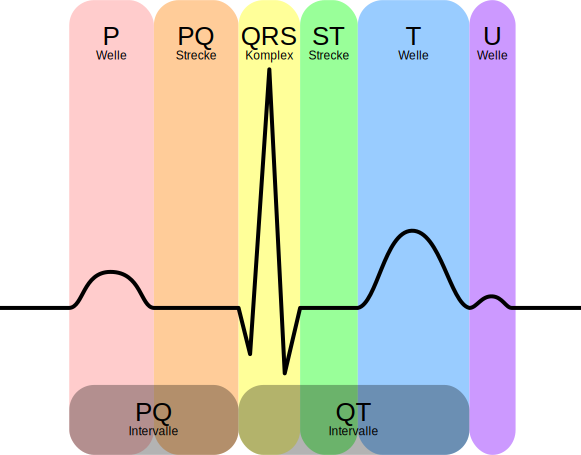
\includegraphics[width=9cm]{./img/EKG_Complex_de}
	\caption{Schematische Darstellung eines EKG eines gesunden Menschen \cite{ekg_symbolic}} \label{01:Wellen-Gesamterregung-Beschriftet}
\end{figure}

\section{Beurteilungsalgorithmus}
Bei der Beurteilung eines EKG's wird nach einem Schema vorgegangen. Bei diesem Schema werden die im folgenden aufgelisteten Punkte abgearbeitet.

\subsection{Frequenz}
Anhand aller Ableitungen wird die Frequenz der Erregungen beurteilt. Dabei ist eine längere Aufnahme einer Ableitung von Vorteil (z.B. die bei manchen EKG-Geräten durchgezogene II-Ableitung). Zur Abschätzung der Frequenz können die großen Kästchen zwischen zwei aufeinanderfolgenden QRS-Komplexen gezählt werden. Mit dem Zählen der großen Kästchen erhält man eine Frequenz von $300 - 150 - 100 - 75 - 60 - 50\ (- 43 - 37.5)$ Erregungen pro Minute.\\
Zusätzlich sollten hier Arrhythmien bereits auffallen. Wenn die Erregung unregelmäßig auftritt kann zusätzlich die Durchschnittliche Frequenz ermittelt werden. Eine Möglichkeit dafür ist es mit den selben Zählschritten ($300 - 150 - ...$) immer drei große Kästchen zu zählen bis man den dritten Komplex erreicht (Anstelle der Zahl drei kann bei Bedarf auch ein beliebiges anderes Vielfaches verwendet werden).

\subsection{Rhythmus}
Es wird untersucht ob ein Sinus-Rhythmus vorliegt bzw. wenn nicht woher der Rhythmus sonst stammt. Auf das Vorliegen eines Sinus-Rhythmus deuten eine gleichbleibende PQ-Zeit sowie eine Frequenz $>\SI{60}{\per\minute}$.
Liegt kein Sinus-Rhythmus vor, springen der AV-Knoten sowie weiter unten liegende Komponenten der Erregungsleitung ein. Der AV-Knoten erzeugt einen Takt mit einer Frequenz von $\num{40}-\SI{50}{\per\minute}$.

\subsection{Intervalle und Zeiten}
Die zeitlichen Abstände zwischen den einzelnen Wellen bzw. deren Breite können Aufschluss auf diverse Probleme geben.

\subsubsection{PQ-Zeit}
Die PQ-Zeit (im Englischen auch PR-Interval genannt) ist die Zeit vom Beginn der P-Welle bis zum Beginn des QRS-Komplexes (siehe Abb. \ref{01:Wellen-Gesamterregung-Beschriftet}). Diese Zeit sollte kleiner als $\SI{0.2}{\second}$ sein.

\subsubsection{QRS-Breite}
Die QRS-Komplexe nennt man 'schmal' wenn sie kleiner als 2.5 kleine Kästchen sind und breit wenn sie diese Grenze überschreiten.

\subsubsection{QT-Zeit}
Die QT-Zeit ist die Zeit vom Beginn des QRS-Komplexes bis zum Ende der T-Welle. Überschreitet diese Zeit einen bestimmten Grenzwert besteht ein erhöhtes Todesrisiko. Dieser Grenzwert beträgt für Frauen $\SI{0.45}{\second}$ und für Männer $\SI{0.47}{\second}$. Allerdings gelten diese Werte nur für eine Herzfrequenz von $\SI{60}{\per\second}$. Um eine Aussage über die QT-Zeit bei anderen Herzfrequenzen treffen zu können kann man die sog. korrigierte QT-Zeit QTc berechnen. Für diese Korrektur gibt es diverse Formeln die jedoch meist nicht für eine Kopfrechnung geeignet sind, allerdings geben die meisten EKG-Geräte QTc aus. Wichtig ist, dass die meisten Korrekturen nur in einem beschränkten Bereich gelten, d.h. die Beurteilung von QTc ist bei sehr hohen und sehr niedrigen Frequenzen kaum möglich.

\subsection{Beurteilung des Lagetyps} \label{01:Lagetyp}


Trägt man die Extremitätenableitungen in der Frontaleben auf erhält man den sog. Cabrerakreis (siehe Abb. \ref{01:Cabrerakreis}). Mithilfe dieses Diagramms kann man die Hauptausbreitungsrichtung der elektrischen Erregung, die sog. elektrische Herzachse bestimmen. Diese ist diagnostisch relevant, da es einerseits Lagetypen gibt die von vornherein als pathologisch (krank) gelten und andererseits da bestimmte Herzerkrankungen die Lage der elekt. Herzachse verändern. Es werden die folgenden Lagetypen unterschieden:
\begin{itemize}
	\item Überdrehter Linkstyp: $\ang{-150}$ bis $\ang{-30}$
	\item Linkstyp: $\ang{-30}$ bis $\ang{30}$
	\item Indifferenz-/Normtyp: $\ang{30}$ bis $\ang{60}$
	\item Steiltyp: $\ang{60}$ bis $\ang{90}$
	\item Rechtstyp: $\ang{90}$ bis $\ang{120}$
	\item Überdrehter Rechtstyp: $\ang{120}$ bis $\ang{210}$
\end{itemize}



\begin{figure}[H]
	\centering
	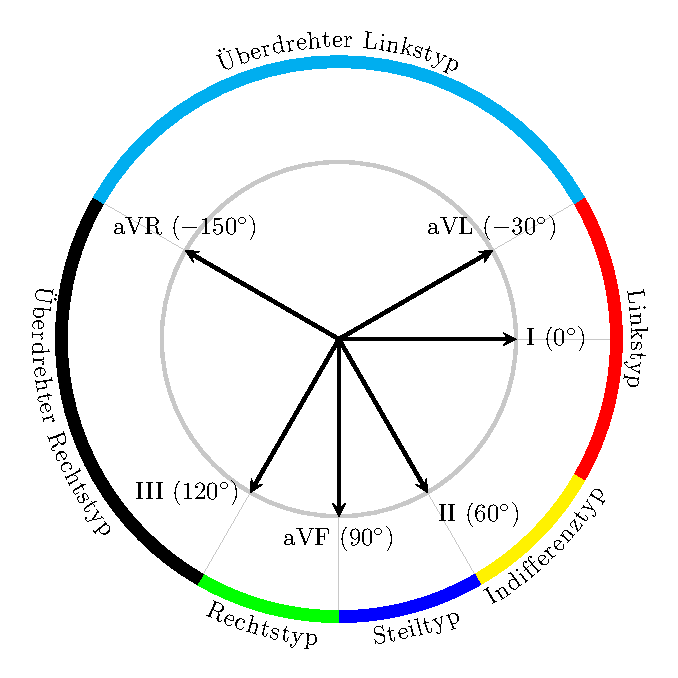
\includegraphics[width=10cm]{./img/Cabrerakreis}
	\caption{Extremitätenableitungen in der Frontalebene (Cabrerakreis)}\label{01:Cabrerakreis}
\end{figure}

Es gilt nun also Anhand der EKG-Kurven der Extremitätenableitungen den ungefähren Winkel der elektrischen Herzachse zu bestimmen. Trägt man die Hauptausbreitungsrichtung der Erregung in ein Diagramm wie Abb. \ref{01:Cabrerakreis} ein, sieht man auf den Ableitungen die Projektion des Vektors der elektr. Herzachse auf den der jeweiligen Ableitung. 

\exkbox{
\textbf{Exkurs: Vektorprojektion}\\
Vereinfacht dargestellt ist ein Vektor ein Pfeil in eine Richtung mit einer bestimmten Länge. Die Projektion eines Vektors $\vec{a}$ auf einen anderen Vektor $\vec{b}$ (Vektorprojektion) ist der Schatten den $\vec{a}$ auf $\vec{b}$ wirft wenn das Licht senkrecht zu $\vec{b}$ steht.
\begin{figure}[H]
	\centering
	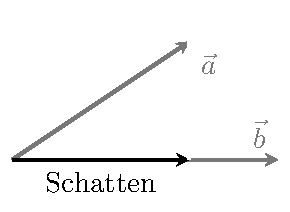
\includegraphics{./img/Vektorprojektion}
	\caption{Vektorprojektion von $\vec{a}$ auf $\vec{b}$.} \label{01:Exk-Vektorprojektion}
\end{figure}
Wenn der Winkel zwischen $\vec{a}$ und $\vec{b}$ mehr als $\ang{90}$ beträgt kommt es zu folgendem Spezialfall:
\begin{figure}[H]
	\centering
	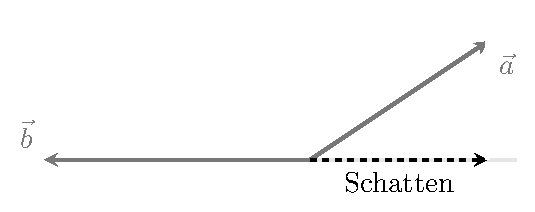
\includegraphics{./img/Vektorprojektion-negativ}
	\caption{Der Spezialfall der negativen Vektorprojektion} \label{01:Exk-Vektorprojektion-negativ}
\end{figure}
Die Projektion von $\vec{a}$ auf $\vec{b}$ zeigt in die selbe Richtung wie $\vec{b}$ (Ausnahme: Im negativen Spezialfall zeigt sie exakt in die Gegenrichtung). 
}
Genauer gesagt sieht man in den QRS-Komplexen der jeweiligen Ableitungen das Vorzeichen und die Länge der Projektion.
\begin{figure}[H]
	\centering
	\ECG{?Positiv, i80, q31, r712, s21, i80, ?Negativ, i80, r31, s712, r21, i80, ?{Neutral (0)}, i80, r55, s55, i80}
\caption{'Positiver', 'Negativer' und 'Neutraler' QRS-Komplex in einer Ableitung} \label{01:Wellen-Vorzeichen}
\end{figure}
Das Vorzeichen zeigt sich wie in Abb. \ref{01:Wellen-Vorzeichen}, die Länge zeigt sich als Höhe der R- bzw. S-Zacken (höhere Zacken bedeuten eine längere Projektion).

\bspbox{
\textbf{Beispiel: Bestimmung des Lagetyps}\\
Zur Veranschaulichung ein Beispiel eines Normaltypen:
\begin{figure}[H]
	\centering
	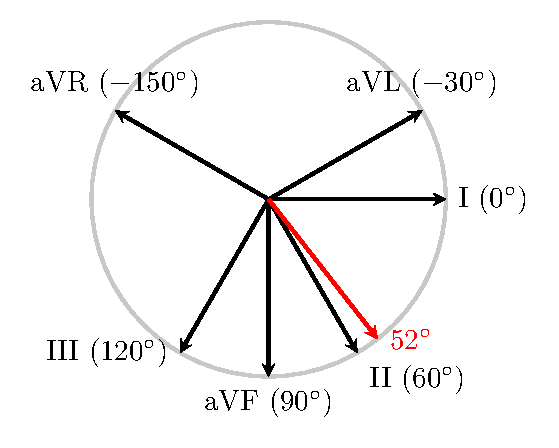
\includegraphics[width=7cm]{./img/Bsp-Lagetyp}
	\caption{Cabrerakreis bei einem Menschen mit Normaltyp}\label{01:Bsp-Lagetyp}
\end{figure}

Bei einem Winkel der elekt. Herzachse von $\ang{52}$ sind die Projektionen auf I, II und aVF deutlich positiv. Deutlich am höchsten ist die R-Zacke in II. aVL steht nachezu negativ auf die elekt. Herzachse und weist damit neutrale Komplexe auf. Ähnlich sieht III aus, allerdings sind dort die Komplexe noch leicht positiv. aVR ist beinahe gegenüber der elekt. Herzachse und hat damit negative Komplexe deren S-Zacken beinahe so hoch sind wie die R-Zacken in II.

\begin{figure}[H]
	\begin{ecg}
		\ECG{?I, i80, !{pp0160}, i40, q21, r66, q11, i50, tp31, 
			?aVR, i80, !{pn0160}, i40, r21, s613, r11, i50, tn33}
		\ECG{?II, i80, !{pp0160}, i40, q21, r615, q11, i50, tp33, 
			?aVL, i80, !{pp0160}, i40, r34, q34, i50, tp31}
		\ECG{?III, i80, !{pp0160}, i70, r35, q33, i50, tp31, 
			?aVF, i80, !{pp0160}, i40, q21, r69, q11, i50, tp32}
	\end{ecg}
	\caption{Symbolisches EKG-Bild zu Abb. \ref{01:Bsp-Lagetyp}} \label{01:EKG,Bsp-Lagetyp}
\end{figure}
}

%TODO Lew 4 quadranten typen

\subsection{LVH (Linksventrikuläre Hypertrophie)}
LVH ist eine pathologische Veränderung des Herzen die meist durch chronische arterielle Hypertonie auftritt. Durch den dauerhaft hohen Blutdruck muss die linke Herzhälfte mehr Leistung bringen wodurch sich der Muskel verdickt (er wird trainiert). Da jedoch die Koronargefäße nicht mitwachsen kann dies u.a. zu einer Mangelversorgung des Herzmuskels (Myokard) führen. Bei der Beurteilung einer EKG-Aufnahme ist der Hauptgrund für die Suche nach Zeichen einer LVH aber, dass diese das Bild stark verändert und damit ev. Diagnosen verfälschen kann. Starke Indikatoren für das Vorhandensein einer LVH  sind:
\begin{itemize}
	\item \textbf{Ein Sokolov-Lyon-Index größer gleich $\mathbf{35}$mm}\\
	Der Sokolov-Lyon-Index ist die Summe der Höhe des tiefsten S-Peaks in V1 oder V2 und des höchsten R-Peaks in V5 oder V6. Dieses Kriterium ist nur anwendbar bei Personen über 35 Jahren
	
	\item \textbf{R in aVL größer gleich $\mathbf{12}$mm}
	
	\item \textbf{Auftreten von LV Strain Pattern in den lateralen Ableitungen (V4-V6, I \& aVL)}\\
	Ein LV Strain Pattern ist eine (absinkende) ST-Senkung in Kombination mit einer negativen T-Welle.
	
	\item \textbf{Drehung der elekt. Herzachse nach Links}\\
	Bei LVH liegt, aufgrund des vergrößerten Linksherzes, meist ein Linkstyp oder ein überdrehter Linkstyp vor.
\end{itemize}

\bspbox{
	\textbf{Beispiel: Linksventrikuläre Hypertrophie}\\
	Im folgenden Bild ist erkennbar, dass von den Extremitätenableitungen der größte R-Peak in I liegt. Zusätzlich ist aVF neutral bis leicht negativ. Dies lässt auf einen Winkel der elekt. Herzachse leicht unter $\ang{0}$ schließen und ergibt somit einen Linkstyp. Der niedrigste S-Peak in V1 oder V2 und der höchste R-Peak in V5 oder V6 ergeben in Summe $\SI{61}{\milli\meter}$ und liegen damit deutlich über $\SI{35}{\milli\meter}$. Die R-Peaks in aVL sind mit $\SI{14}{\milli\meter}$ größer als $\SI{12}{\milli\meter}$ und sowohl in V5 als auch in V6 ist ein LV strain pattern erkennbar. Es sind alle oben erwähnten Indikatoren vorhanden, eine LVH ist damit sehr wahrscheinlich.
	\begin{figure}[H]
		\centering
		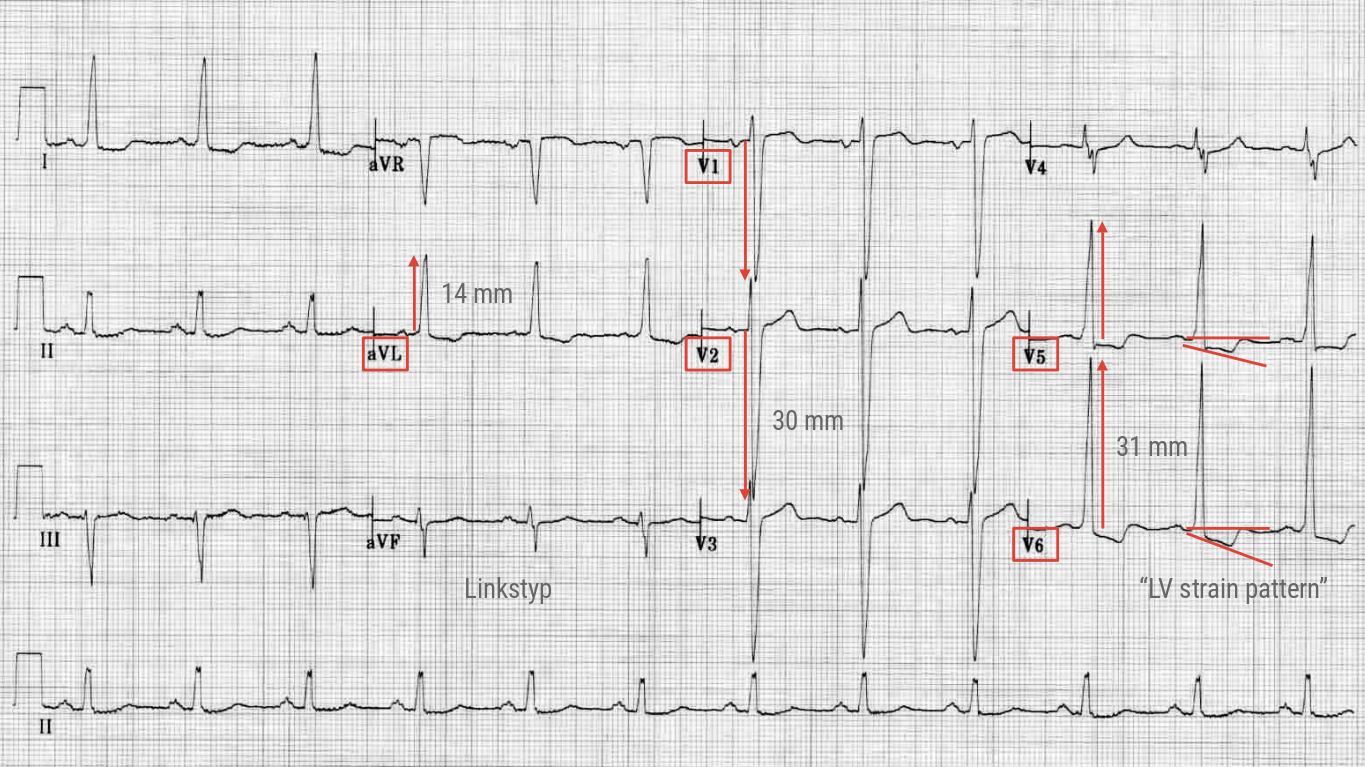
\includegraphics[width=0.95\textwidth]{./img/Bsp-LVH}
		\caption{12-Kanal EKG eines Patienten/einer Patientin mit LVH}\label{01:Bsp-LVH}
	\end{figure}

}

%TODO
%\nuovoECG{lvstrain1}{(0,0)--(0.02,-0.1)--(0.4,-0.12)--(0.43,-0.13)--(0.45,-0.14)--(0.47,-0.142)--(0.49,-0.13)--(0.5,-0.125)--(0.65,0)}
%\begin{figure}[H]
%	\begin{ecg}
%		\ECG{?I, i80, !{pp0160}, i70, r917, !{lvstrain1}, i40}
%	\end{ecg}
%	\caption{Symbolisches EKG-Bild zu Abb. \ref{01:Bsp-Lagetyp}} \label{01:EKG,Bsp-Lagetyp}
%\end{figure}

\newpage
\section{Erregungsleitung}
Im gesunden Herz geht die Erregung vom Sinusknoten im Vorhof aus. Beim Eintreffen im AV-Knoten wird sie kurz verzögert, um dem Atrium (Vorhof) Zeit zu geben. Vom AV-Knoten breitet sich die Erregungsleitung über das His-Bündel in den linken und den rechten Tawaraschenkel aus. Der Linke Tawaraschenkel teilt sich, weil das Linksherz größer ist, noch in einen hinteren (posterioren) und vorderen (anterioren) Teil.
\begin{figure}[H]
	\centering
	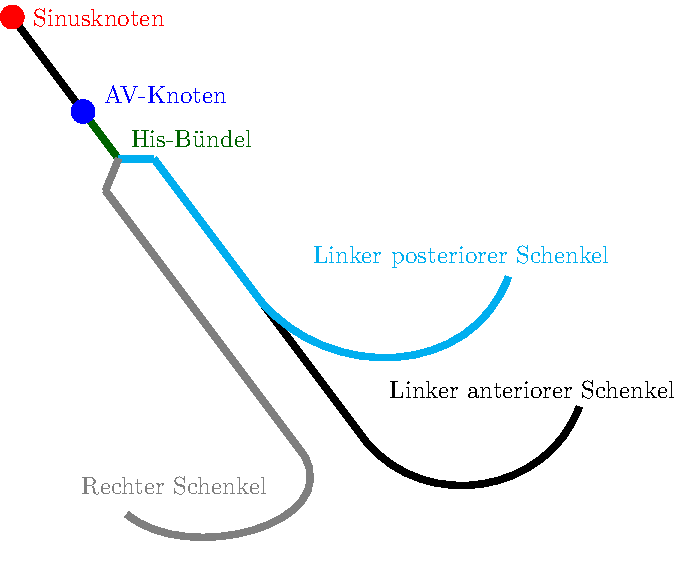
\includegraphics[width=8cm]{./img/Erregungsleitung}
	\caption{Erregungsleitungssystem des menschlichen Herzen (vereinfacht).}\label{01:Erreigungsleitungssystem}
\end{figure}
Der Sinusknoten erzeugt, vom Nervensystem gesteuert, mit einer Frequenz von mehr als $\approx\SI{60}{\per\minute}$ ein Signal. Der AV-Knoten erzeugt ebenfalls mit einer Frequenz von $\approx\num{40}-\SI{50}{\per\minute}$ ein Signal, allerdings wird dieses unterdrückt, wenn zwischenzeitlich eine Erregung vom Sinusknoten ankommt. Durch die niedrigere Frequenz führt dies dazu, dass beim Ausfall des Sinusknoten bzw. der Erregungsleitung zum AV-Knoten dieser die Schrittmacherfunktion des Herzes übernimmt. Eine ähnliche Funktion gibt es auch im His-Bündel mit einer Eigenfrequenz von $\approx\num{20}-\SI{30}{\per\minute}$ bzw. Des Weiteren kann auch jede Herzmuskelzelle mit einer niedrigen Frequenz ein Signal erzeugen. Ist die Schrittmacherfunktion oder Erregungsleitung in diesem System gestört kommt es zu verschiedenen Pathologien.

\subsection{Atrioventrikulärer Block (AV-Block)}
Wie der Name schon vermuten lässt handelt es sich hierbei um ein Problem/eine Blockade bei der Überleitung der Erregung vom Atrium (Vorhof) in den Ventrikel (Kammer). Abhängig von der Symptomatik unterscheidet man 3 Grade von AV-Blocks.

\subsubsection{AV-Block I\textdegree\ (Grad 1)}
Bei einem AV-Block vom Grad ist die Überleitung vom Atrium (Vorhof) in den Ventrikel (Kammer) stärker verzögert. Am EKG macht sich das durch eine PQ-Zeit $>\SI{0.2}{\second}$ bemerkbar. Er bleibt meist symptomlos und ist damit klinisch kaum relevant.

\subsubsection{AV-Block II\textdegree\ (Grad 2)}
Beim AV-Block II\textdegree\ kommt es trotz vorhandener Atriumserregung zum teilweisen Ausfall der Kammerkontraktion. Es werden zwei Typen von AV-Block II\textdegree\ unterschieden.
\paragraph{AV-Block II\textdegree\ Typ 1 (Wenckeback / Mobitz 1)}
Bei diesem Typ von AV-Block wird (meist durch Zellermüdung) die PQ-Zeit mit jeder Erregung länger bis die Kammeraktion einmalig ausfällt. Dadurch wird die PQ-Zeit wieder zurückgesetzt. Die Erregung ist rhythmisch arrhythmisch.
\begin{figure}[H]
	\begin{ecg}
		\ECG{i40, !{pp0160}, i60, q31, r510, s21, i50, tp22, i210,
			!{pp0160}, i120, q31, r510, s21, i50, tp22, i150,
			!{pp0160}, i180, q31, r510, s21, i50, tp22, i90,
			!{pp0160}, i620,
			!{pp0160}, i60, q31, r510, s21, i50, tp22, i210,
			!{pp0160}, i120, q31, r510, s21, i50, tp22, i150,
			!{pp0160}, i180, q31, r510, s21, i50, tp22, i90,
			!{pp0160}, i620}
	\end{ecg}
	\caption{AV-Block II\textdegree\ Typ 1} \label{01:EKG-AV-Grad2-Wenckebach}
\end{figure}

\paragraph{AV-Block II\textdegree\ Typ 2 (Mobitz / Mobitz 2)}
Bei einem AV-Block II\textdegree\ Typ 2 bleibt die PQ-Zeit konstant und die AV-Überleitung funktioniert ein- bis mehrmals korrekt, anschließend fällt die Kammererregung ein- bis mehrmals aus. Bei dieser Art von AV-Block wird das Verhältnis von Erregungen im Atrium zu den Erregungen im Ventrikel angegeben. Im Spezialfall des 2:1-Blocks (es kommen 2 P-Wellen auf jeden QRS-Komplex) ist es nicht möglich Typ 1 und Typ 2 zu unterscheiden, diese Art von Block nennt man 2:1 AV-Block. Die Erregung ist ebenfalls rhythmisch arrhythmisch.
\begin{figure}[H]
	\begin{ecg}
		\ECG{i40, !{pp0160}, i60, q31, r510, s21, i50, tp22, i210,
			!{pp0160}, i60, q31, r510, s21, i50, tp22, i210,
			!{pp0160}, i620,
			!{pp0160}, i60, q31, r510, s21, i50, tp22, i210,
			!{pp0160}, i60, q31, r510, s21, i50, tp22, i210,
			!{pp0160}, i620,
			!{pp0160}, i60, q31, r510, s21, i50, tp22, i210,
			!{pp0160}, i60, q31, r510, s21, i50, tp22, i210
			}
	\end{ecg}
	\caption{AV-Block II\textdegree\ Typ 2 (3:2)} \label{01:EKG-AV-Grad2-Mobitz}
\end{figure}

\subsubsection{AV-Block III\textdegree\ (Grad 3)}
Bei einem AV-Block III\textdegree\ ist die Überleitung vom Atrium in den Ventrikel komplett blockiert, Der Sinus- und der AV-Knoten geben unabhängig von einander den Takt für das Atrium und den Ventrikel vor. Am EKG ist dies daran zu erkennen, das kein Zusammenhang zwischen P-Wellen und den Kammerkomplexen besteht.

\nuovoECG{avblock3-tp-overlap}{(0, 0) -- (0.1, 0.07) -- (0.2, 0.19) -- (0.25, 0.18) -- (0.3, 0.235) -- (0.355, 0.184) -- (0.38, 0.13) -- (0.4, 0.06) -- (0.45, 0.03) -- (0.5, 0)}

\nuovoECG{avblock3-rp-overlap}{(0, 0) -- (0.0625, 1) -- (0.11, 0.12) -- (0.12, 0.1) -- (0.14, 0.08) -- (0.16, 0)}

\begin{figure}[H]
	\begin{ecg}
		\ECG{i40, 
			!{pp0160}, r510, s21, i50, tp22, i500,
			!{pp0160}, i200, r510, s21, i50, tp22, i300,
			!{pp0160}, i400, r510, s21, i50, tp22, i100,
			!{pp0160}, i600, r510, s21, i60, !{avblock3-tp-overlap}, i620,
			i130, !{avblock3-rp-overlap}, i25, tp22, i500
			}
	\end{ecg}
	\caption{AV-Block III\textdegree} \label{01:EKG-AV-Grad3}
\end{figure}

\subsection{Schenkelblock}
Ist die Erregungsleitung in einem der Schenkel blockiert, läuft die Erregung vom anderen, normal funktionsfähigen, Schenkel über das Myokard zum gestörten Teil des Herzen, Da jedoch die Erregungsleitung im Myokard deutlich langsamer verläuft als in den Schenkeln, macht sich eine derartige Störung durch breite QRS-Komplexe bemerkbar. Ab einer Breite von $\SI{0.12}{\second}$ (3 kleine Kästchen) spricht man von einem kompletten Schenkelblock.

\subsubsection{Rechtsschenkelblock}
Wenn der Rechte Schenkel blockiert ist, wird zuerst das Linksherz über den Linken Schenkel erregt und anschließend über das Moykard das Rechtsherz. Dadurch wird am EKG während der Komplexe ein, zeitlich 'breiter', 'Strom' von Links nach Rechts sichtbar. D.h. Anteriore (frontale) Ableitungen (V1 \& V2) zeigen deutlich positive Komplexe. Typisch sind auch die sog. Hasenohren: eine kleine, schmale r-Zacke direkt gefolgt von einer großen breiten R'-Zacke. Bei den lateralen (seitliche, beim ELG immer links) Ableitungen (V4-V6, I, aVL) zeigen sich deutlich breitere zum Teil auch stumpfe S-Zacken.

\nuovoECG{hasenohren}{(0,0) -- (0.05, 0.3) -- (0.1, -0.08) -- (0.2, 0.6) -- (0.3, 0.9) -- (0.4, 0)}
\nuovoECG{abstand}{(0,0) (0.4, 0)}
\nuovoECG{breite-s}{(0,0) -- (0.01, -0.3) -- (0.25, 0)}
\nuovoECG{stumpfe-s}{(0,0) -- (0.01, -0.3) -- (0.1, -0.32) -- (0.2, -0.32) -- (0.25, 0)}
\begin{figure}[H]
	\centering
	\begin{minipage}[b]{0.2\textwidth}
		\centering
		\begin{ecg}
			\ECG{i40, !{pp0160}, i60, !{hasenohren}, i40, tn23, i80}
		\end{ecg}
		\subcaption{'Hasenohren'}\label{01:EKG-RSB-Hasenohren}
	\end{minipage}%
	\begin{minipage}[b]{0.3\textwidth}
		\centering
		\begin{ecg}
			\ECG{i40, !{pp0160}, i60, r39, !{breite-s}, i60, tp22, i80, !{abstand}, 
				i40, !{pp0160}, i60, r39, !{stumpfe-s}, i60, tp22, i80}
		\end{ecg}
		\subcaption{\centering Breite/Stumpfe S-Zacken} \label{01:EKG-RSB-Breite-S}
	\end{minipage}
\end{figure}

\bspbox{
	\textbf{Beispiel: Rechtsschenkelblock}\\
	Im folgenden Bild sind in V1 und V2 die doppelten R-Zacken (rSR'-Komplexe, Hasenohren) zu erkennen, ebenfalls sichtbar ist, dass die lateralen Ableitungen (I, aVL, V4-V6) sowie hier auch II breite, stumpfe S-Zacken aufweisen. In Kombination mit den in allen Ableitungen breiten Komplexen lässt sich auf einen Rechtsschenkelblock schließen.
	\begin{figure}[H]
		\centering
		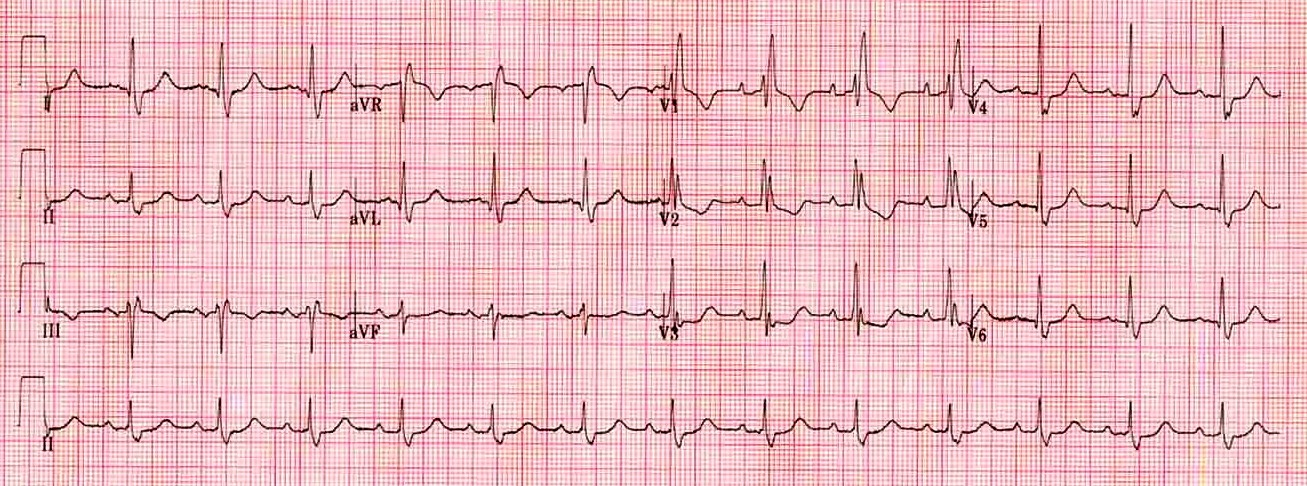
\includegraphics[width=0.95\textwidth]{./img/Bsp-RBBB}
		\caption{12-Kanal EKG eines Patienten/einer Patientin mit Rechtsschenkelblock \cite{ekg_rbbb}}\label{01:Bsp-RBBB}
	\end{figure}
}

\subsubsection{Linksschenkelblock}
Beim Linksschenkelblock ist der Vorgang umgekehrt, d.h. die Erregung verläuft über den funktionsfähigen rechten Schenkel und breitet sich vom Rechtsherz über das Myokard zum Linksherz aus. Dadurch ist am EKG eine Bewegung von rechts nach links sichtbar. Anteriore Ableitungen zeigen kaum vorhandenen r-Zacken gefolgt von tiefen und breiten S-Zacken. Die lateralen Ableitungen weisen breite, stumpfe R-Zacken und eine ST-Senkung in Kombination mit einer negativen T-Welle auf.



\appendix
\newpage
\section{Quellen \& OpenSource Code}

\subsection{LaTex Paket: ecgdraw}
Die in diesem Dokument gezeigten symbolischen EKG-Kurven wurden mit dem LaTeX-Packet ecgdraw von Ezio Aimé und Marco Scavino generiert. Dieses wird mit TeXLive und MikTex standardmäßig ausgeliefert. Mehr Informationen dazu finden sich unter \url{https://ctan.org/pkg/ecgdraw?lang=en}


\newpage
\bibliographystyle{plain}
\bibliography{./content/bibliography}

\end{document}
